\chapter{Matching Local Image Features}

In this chapter we will introduce local feature points in images and 
explain how they are used. We will start out by discussing why we need 
local features in the first place before looking at the inner workings 
of modern local image features. Finally we will look at how they are 
used, in particular how corresponding pairs are found in between two or 
more images.

\section{A Brief Look at Computer Vision}

The field of computer vision is anecdotally said to have been founded 
when Marvin Minsky assigned the problem of making a computer see as an 
undergraduate summer project back in 1966\footnote{This is the same 
Marvin who invented neural networks and went on to serve as scientific 
adviser on Kubrick's movie \emph{Space Odyssey 2001}}. Whether or not 
the anecdote is true, the idea that the field of computer vision should 
be solvable in a summer's worth of time but still to this days remains 
an active field of research, illustrates an interesting notion: Making 
computers solve tasks involving seeing turns out to be much harder than 
we would initially assume.

Part of this notion stems from the fact that vision is a problem that we 
as humans are very good at. We can easily recognize objects under 
different light, or stitch together photographies to a panorama, or 
navigate a corridor identifying obstacles along the way. In fact these 
things are so easy to us, that it seems strange that they should be 
difficult at all, yet consistently recognizing an object under different 
lighting conditions and from different angles can still cause problems 
for even the best object recognition algorithms.

\subsection{A Thought Experiment}

The main factor that makes computer vision difficult is how the world we 
see around us constantly varies. This is not something that is 
immediately obvious to the casual observer, so for the sake of clarity 
let us do a small thought experiment. Try for a moment to imagine that 
you enter a room and recognize the newspaper that is lying on the table, 
illuminated from the grey light coming in of the window on the opposing 
wall. You move across the room and switch on the light make out if the 
paper is from today, and then you sit down and put on your glasses to 
read the headline. Try to imagine the newspaper as you see it on three 
different stages. First as you enter the room, then as you turn after 
turning on the light, now standing on the other side of the table, and 
last when you are sitting with the paper in your hand after you put on 
your glasses. For each of these stages, picture the situation as a 
photography and look at how the newspaper changes as you move around. At 
first you see it at an angle lying in a fairly dark and grey room, the 
white pages reflecting the light from the window with a cold bluish hue 
and the words too far away to make out. Then in the second stage with 
light on, the object you are looking at has suddenly changed. When you 
turned on the light in the room, you also changed the color of the 
newspaper, which now has a warm and yellowy white color.  The angle you 
are looking at the paper from has changed too, and the words and 
pictures are no longer upside down, although still slightly rotated and 
with the increased light in the room the contrast of the words and 
pictures of the page makes it possible for you to make recognize that 
the newspaper is from today. Finally as you sit down and put your 
glasses on the newspaper changes again. The color might be the same, but 
if you imagine taking a photography as you are sitting with the paper in 
your hand, the newspaper will look much bigger almost taking up the 
entire frame. Now that your glasses are on, the words stand out much 
clearer and you can see what is in the pictures on the front page.

Intuitively you know that the paper you sat down to read is the same 
object as the paper you saw when you entered the room, but if we limit 
ourselves to only looking at the object itself, almost everything about 
it changed in the process, from the color of the pages to the sharpness 
of the lines. On top of that the paper has changed in size and rotation 
from lying on the table to being in your hand. In our daily lives we are 
aided in the process of recognizing the paper by our memory and idea of 
how the world works. When we walked in to the dark room and saw 
something on the table, it was probably safe to assume that it was a 
newspaper. Maybe the newspaper always lies like that on the table, or 
maybe we left it there ourselves. Afterwards as we move around in the 
room, we can safely assume that the paper didn't move and even if it 
might not look exactly the same after we turned on the light, it's safe 
to guess that nobody took the old newspaper and replaced it with a new 
and yellower version.

On the other hand a computer algorithm trying to recognize objects will 
not be able to make the same assumptions about the world. We might just 
give as input to the program to pictures of the newspaper. One from the 
first stage where the light was turned off, the paper was far away and 
the lens wasn't focused correctly, and one from the third stage with the 
light on, the image in focus and the paper taking up the entire photo.  
Now we ask the algorithm: "Is this the same newspaper?". In this case it 
is fair to ask how the algorithm can reliably make this judgement.

\section{Introducing Local Features}

The example of the newspaper focuses on a particular branch of computer 
vision; object recognition, but the exact same problem remains for most 
of the various subfields. In automatic panorama stitching where we try 
to create a panorama from a set of images, we need to recognize which 
images fit together even if they are taken with different camera 
settings. In near duplicate detection where we try to find images that 
appear to be duplicates of other images we need to recognize if the same 
scene appears from slightly different angles under slightly different 
light. In scene matching where we try to find out if two images are 
taken of the same scene the two images could be taken on different days 
under different conditions. The list continues and it should hopefully 
be clear that in order to solve a lot of problems in computer vision, we 
need a way to deal with these variations.

One particularly successful approach over recent years has been to use 
\emph{local image features}. As opposed to global image features like 
the image histogram or the position of edges, local features are each 
constrained to a small point-like area in the image. The idea behind 
local features is that we pick distinct points in the image and describe 
the local neighborhood in a way that remains stable even if the image is 
taken under different light or from slightly different angles. Then 
given two images we can find some local feature points of each and see 
if any correspond across images.

\begin{figure}[t]
	\centering
	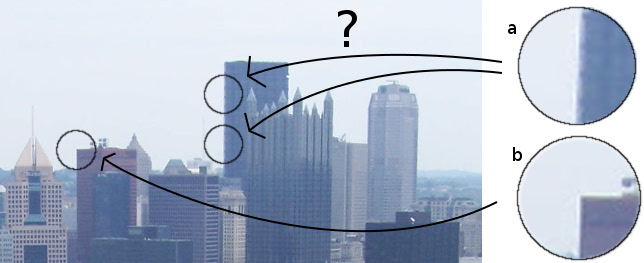
\includegraphics[width=1\columnwidth]{images/feature_point}
	\caption{Example of feature point location. In the image, feature a) 
is ambiguous because it can match any location along the left edge of 
the building, while feature b) is distinct because only one left corner 
of that building exists. The background image is originally from the 
Gallagher dataset \cite{gallagher2008}}
	\label{fig:feature_point}
\end{figure}

For this two work we need two components. First we need to find spots in 
an image that are distinct, since if we have similar points we can't 
uniquely match them. Secondly we need to take information around the 
local area of the point and describe it in a way that is invariant to 
changes like illumination and geometric distortion as well as noise, 
blur and scale. Finding unique points in the image is called 
\emph{feature detection} and it yields a \emph{key point}, where as we 
describe the key point with a \emph{feature descriptor}. The key point 
will contain the position of the point in the image while the descriptor 
will contain information about the image data surrounding that position.

\subsection{Finding Feature Points}

As Figure~\ref{fig:feature_point} illustrates, an easy heuristic for 
finding a unique point in an image is to find corners. A point lying on 
a smooth part of the image would look identical to the surrounding 
points, and points along an edge will look the same as other points 
along the same edge. While corners aren't necessarily a sufficient 
condition for finding a good feature point, they provide a good starting 
point. Intuitively the simplest way to find corners would be to detect 
edges in the image (for example using a high pass filter), and follow 
these edges until they turn. Some of these approaches are detailed in 
\cite{university1978comparison}. 

A different (and it turns out, better) approach is to look at the 
gradient across the image and find spots where there is a gradient in 
two perpendicular directions.  That is, along a dark edge on a bright 
background there will be a gradient perpendicular to the edge, but no 
gradient along the edge.  However in a corner we would have a gradient 
in two different directions. The idea was originally introduced by 
Morevec \cite{hans1977towards} and later improved upon by Harris and 
Stephens who introduced what is now commonly known as the Harris corner 
detector \cite{harris1988combined}.

Alternatively a fast way of deciding if a point is a corner is to look 
at all pixels surrounding the point of interest and compute the fraction 
of pixels that have higher intensities than the center\footnote{i.e.\ 
are brighter}. We can then find corners by thresholding on this 
intensity difference as proposed by Smith and Brady 
\cite{smith1997susan} as the SUSAN edge detector. Lepetit and Fua 
proposed a similar algorithm but only looking at the pixels on the 
circumference of a circle surrounding the point 
\cite{lepetit2006keypoint}. This is also the central idea behind the 
FAST detector by Rosten and Drummond \cite{rosten2006machine}.

For a thorough review of the history of feature detectors, Tuytelaars 
and Mikolajczyk presents an excellent historical retrospect in 
\cite{tuytelaars2008local}.

\subsection{Describing Feature Points}

Once we have found a point of interest, we need to describe it. The 
simplest way is to save the values of the pixels in the immediate 
neighborhood, but this would not be very flexible. Take the case where 
we take two images of the same scene, but overexpose one of them. Two 
corresponding feature points would not look remotely alike in this case.
In the feature descriptor of bright photography all the pixel values 
would be high, while the values in the descriptor of the darker image 
would all be low. A similar situation arise if one image is rotated or 
there is a change in perspective.

A way to work around these issues is to compile a histogram of the 
pixels surrounding the key point. This way we would get the same 
descriptor now matter how the image is rotated. To a certain extend this
method is also invariant to affine transformations, that is change in 
perspective as long as approximately the same pixels fall within the 
zone we are taking a histogram of. If we use the raw values of the 
pixels, the descriptor is still not invariant with respect to 
brightness, but this is easily solved by creating a histogram of the 
pixel values relative to the center pixel. Lazebnik et al.\ introduced 
this method in \cite{lazebnik2003sparse} adding the distance from the 
key point as another dimension in the histogram.

Instead of using the pixel values, we can create a histogram of the 
gradients surrounding the feature point as Lowe did in his Scale 
Invariant Feature Detector (SIFT) \cite{lowe2004sift}. The histogram he 
proposes is based on the gradient locations and orientations weighted by
the gradient magnitude. To make sure that the histogram is rotation 
invariant, the bins of the histogram are normalized and start with the 
bin of the highest magnitude. The SIFT descriptor has been very widely 
used since it's introduction and has become a de facto standard in 
computer vision. To enhance the computational time needed to compute 
descriptors, Bay et al.\ introduced the Speeded Up Robust Features 
(SURF) that rely on a histogram of wavelets instead of gradients as used 
in SIFT \cite{bay2006surf}. 

A radically different approach to a feature descriptor is to measure the
intensity difference between a number of pixels surrounding the key 
point and simply assign the bits to a vector that is returned as the 
feature descriptor. Calonder et al.\ \cite{calonder2010brief} introduced 
a feature descriptor, Binary Robust Independent Elementary Features 
(BRIEF), based on this idea. The main advantage of their approach is 
reduced processing and memory needed to create, store and match the 
feature descriptors. Interestingly the positions used for pixel wise 
comparisons were selected at random and tested against similar random 
configurations using the configuration yielding the best result. The 
simplicity of this method allows for real time matching of objects from 
a video stream, something that would be too computationally tolling when 
using a descriptor like SIFT\@. BRIEF however fails to be rotation 
invariant making it less useful in cases where images are not 
necessarily upright.

\section{Finding the Perfect Match}

Most applications of feature points use them to match features across 
different images. The standard out of the box way most feature points 
are matched involve comparing the feature descriptor using some kind of 
distance measure. If we match all features of one image with all 
features of another and discard all matches that are below a certain 
threshold of similarity, we have in essence a set of matches between the
two images. For most feature points (for example SIFT and SURF), this 
similarity is measured by the cosine similarity. Binary descriptors such
as BRIEF can take advantage of the faster computation of the hamming 
distance.

\subsection{Geometric Constraints}

While the standard matching method is often computationally efficient, 
it isn't necessarily the best way to match feature points. Many matching 
methods make use of the knowledge of the position of the keypoints in 
the image, i.e.\ the geometrical meta data. Using this information can 
often yield more accurate outcomes, but they inevitably make assumptions
about the geometric relationship between the images that are being 
matched which might not hold true.  

A simple example would be to only consider matches that aren't deviating 
too much with respect to the average angle and distancen as considered 
by \cite{kim2008efficient}.  This performs well in situations where no 
camera rotation occurs between the two images, but fails when this 
assumption isn't met. Various scenarios have been proposed to improve on 
this simple assumption such as epipolar constraints 
(\cite{torr2000mlesac}, \cite{chum2005matching}) and pairwise 
constraints (\cite{choi2009robust}, \cite{leordeanu2005spectral}). The 
Epipolar constraint carries the assumption that the two images matched 
are related by an affine transformation. That is, that there is no 
relative movement of objects in between images and either the viewpoint 
is fixed or the image resides entirely on a plane. In practice this 
assumption largely holds true when all objects we are interested in 
matching are roughly the same distance from the camera given that 
objects don't move across images.  Pairwise constraints provide a more 
robust approach to the same problem by looking at a set of proposed 
correspondences and defining a pairwise error between any two matches 
for example based on the assumption that two neighboring correspondences 
will usually have similar angles and distances. We can then convert the 
problem to an optimization problem and return a set of correspondences 
that minimizes this error such as proposed in \cite{choi2009robust} and 
\cite{leordeanu2005spectral}.  This approach provides more robustness in 
cases where assumptions that are violated globally still hold on a local 
scale.

An alternative is to pick out different areas in each image and pair 
areas when correspondence pairs are mainly found going from one area to 
another. This allows for the filtering of all correspondences that do 
not fall within paired areas. Examples include \emph{Isodata} 
\cite{das2008event}, which clusters feature points according to their 
position in the image, and the method from \cite{wu2011robust}, which 
uses maximally stable extremal regions (MSER) feature points to 
designate areas. 

\subsection{Matching Without Assumptions}

In practice there are many situations where relying on the geometry of 
the image to filter correspondences is not possible, for example images 
without overlap, or adjacent objects in one image are that are separated 
in another. Furthermore, methods using geometric constraints all require 
an initial set of correspondences. If this set of correspondences can be 
narrowed down to the most probable correct matches, the geometric 
matching algorithm will benefit in terms of speed and accuracy.  Finally 
some use cases might require a speed that simply cannot be achieved by 
complex geometric methods.

In the absence of geometric constraints, only few methods are available.  
As pointed out in \cite{szeliski2010} and mentioned above, the simplest 
approach to matching feature points is to return all matches above a 
given threshold of similarity.  This can be done with a fixed threshold 
or by finding the nearest neighbors for each point (still filtering by a 
threshold to avoid including matches for feature points that have no 
counterpart in the other image).  When Lowe \cite{lowe2004sift} proposed 
the scale-invariant feature transform he included an alternative 
matching measure. Instead of rating matching by similarity assessed the 
uniqueness of a given match by looking at the two nearest neighbors of 
each feature point and calculating the matching score as the ratio of 
similarities. This method will later be referred to as \emph{Ratio}.  
Ranking the scores by their uniqueness and picking the $n$ best produces 
a set of correspondences that are distinctly matched across two images.  
Of these three methods (fixed threshold, nearest neighbors, and 
\emph{RATIO}), \emph{RATIO} was found to perform best by a slight margin 
\cite{mikolajczyk2005performance}.

%Matching feature points
% - What applications require matching?
% - How is matching usually done
% - Segue into related work from paper
